% !TEX encoding = UTF-8 Unicode
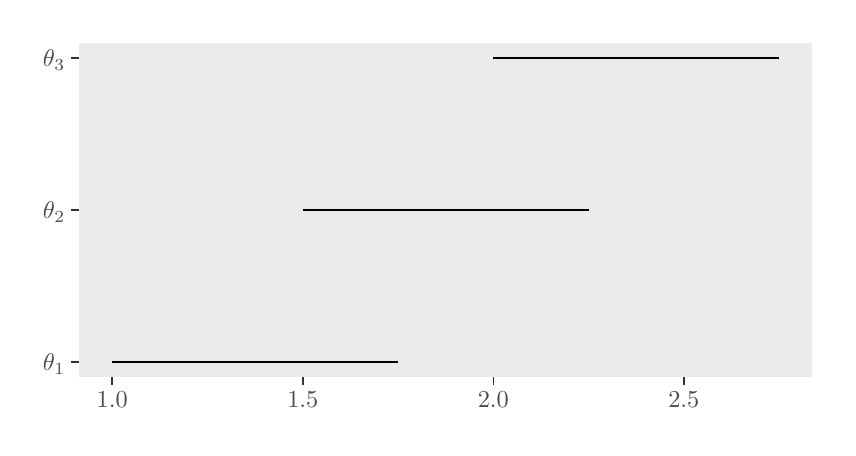
\begin{tikzpicture}[x=1pt,y=1pt]
\definecolor{fillColor}{RGB}{255,255,255}
\path[use as bounding box,fill=fillColor,fill opacity=0.00] (0,0) rectangle (289.08,144.54);
\begin{scope}
\path[clip] (  0.00,  0.00) rectangle (289.08,144.54);
\definecolor{drawColor}{RGB}{255,255,255}
\definecolor{fillColor}{RGB}{255,255,255}

\path[draw=drawColor,line width= 0.6pt,line join=round,line cap=round,fill=fillColor] (  0.00,  0.00) rectangle (289.08,144.54);
\end{scope}
\begin{scope}
\path[clip] ( 18.53, 18.22) rectangle (283.58,139.04);
\definecolor{fillColor}{gray}{0.92}

\path[fill=fillColor] ( 18.53, 18.22) rectangle (283.58,139.04);
\definecolor{drawColor}{RGB}{0,0,0}

\path[draw=drawColor,line width= 0.6pt,line join=round] ( 30.58, 23.71) -- (133.84, 23.71);

\path[draw=drawColor,line width= 0.6pt,line join=round] ( 99.42, 78.63) -- (202.69, 78.63);

\path[draw=drawColor,line width= 0.6pt,line join=round] (168.27,133.55) -- (271.53,133.55);
\end{scope}
\begin{scope}
\path[clip] (  0.00,  0.00) rectangle (289.08,144.54);
\definecolor{drawColor}{gray}{0.30}

\node[text=drawColor,anchor=base east,inner sep=0pt, outer sep=0pt, scale=  0.88] at ( 13.58, 20.68) {$\theta_1$};

\node[text=drawColor,anchor=base east,inner sep=0pt, outer sep=0pt, scale=  0.88] at ( 13.58, 75.60) {$\theta_2$};

\node[text=drawColor,anchor=base east,inner sep=0pt, outer sep=0pt, scale=  0.88] at ( 13.58,130.52) {$\theta_3$};
\end{scope}
\begin{scope}
\path[clip] (  0.00,  0.00) rectangle (289.08,144.54);
\definecolor{drawColor}{gray}{0.20}

\path[draw=drawColor,line width= 0.6pt,line join=round] ( 15.78, 23.71) --
	( 18.53, 23.71);

\path[draw=drawColor,line width= 0.6pt,line join=round] ( 15.78, 78.63) --
	( 18.53, 78.63);

\path[draw=drawColor,line width= 0.6pt,line join=round] ( 15.78,133.55) --
	( 18.53,133.55);
\end{scope}
\begin{scope}
\path[clip] (  0.00,  0.00) rectangle (289.08,144.54);
\definecolor{drawColor}{gray}{0.20}

\path[draw=drawColor,line width= 0.6pt,line join=round] ( 30.58, 15.47) --
	( 30.58, 18.22);

\path[draw=drawColor,line width= 0.6pt,line join=round] ( 99.42, 15.47) --
	( 99.42, 18.22);

\path[draw=drawColor,line width= 0.6pt,line join=round] (168.27, 15.47) --
	(168.27, 18.22);

\path[draw=drawColor,line width= 0.6pt,line join=round] (237.11, 15.47) --
	(237.11, 18.22);
\end{scope}
\begin{scope}
\path[clip] (  0.00,  0.00) rectangle (289.08,144.54);
\definecolor{drawColor}{gray}{0.30}

\node[text=drawColor,anchor=base,inner sep=0pt, outer sep=0pt, scale=  0.88] at ( 30.58,  7.21) {1.0};

\node[text=drawColor,anchor=base,inner sep=0pt, outer sep=0pt, scale=  0.88] at ( 99.42,  7.21) {1.5};

\node[text=drawColor,anchor=base,inner sep=0pt, outer sep=0pt, scale=  0.88] at (168.27,  7.21) {2.0};

\node[text=drawColor,anchor=base,inner sep=0pt, outer sep=0pt, scale=  0.88] at (237.11,  7.21) {2.5};
\end{scope}
\end{tikzpicture}
